%%%%%%%%%%%%%%%%%%%%%%%%%%%%%%%%%%%%%%%%%%%%%%%%%%%%%%%
%%% 可能用到的网站`'
%%%%%%%%%%%%%%%%%%%%%%%%%%%%%%%%%%%%%%%%%%%%%%%%%%%%%%%
%%% LaTeX公式编辑器:https://www.latexlive.com/
%%% Diagram流程图绘制:https://www.drawio.com/
%%%%%%%%%%%%%%%%%%%%%%%%%%%%%%%%%%%%%%%%%%%%%%%%%%%%%%%

%%%%%%%%%%%%%%%%%%%%%%%%%%%%%%%%%%%%%%%%%%%%%%%%%%%%%%%
%%% 模板参数设置
%%%%%%%%%%%%%%%%%%%%%%%%%%%%%%%%%%%%%%%%%%%%%%%%%%%%%%%
\documentclass{mcmthesis}  % 文档类型
\mcmsetup{
        tcn = 12345678,   % 队伍控制号
        problem = ABCDEF,  % 选题
        sheet = true,   % sheet页
        titleinsheet = true,   % sheet页显示标题
        keywordsinsheet = true,  % sheet页显示关键词
        titlepage = false,   % 标题页
        abstract = true  % 摘要
        }
%%%%%%%%%%%%%%%%%%%%%%%%%%%%%%%%%%%%%%%%%%%%%%%%%%%%%%%

%%%%%%%%%%%%%%%%%%%%%%%%%%%%%%%%%%%%%%%%%%%%%%%%%%%%%%%
%%% 导入宏包和引用文献源
%%%%%%%%%%%%%%%%%%%%%%%%%%%%%%%%%%%%%%%%%%%%%%%%%%%%%%%
\usepackage{palatino}  % 帕拉提诺体字体宏包
\usepackage{lastpage}  % 引入 lastpage 宏包
\usepackage{lipsum}  % 导入生成段落的宏包
\usepackage[hyperref=true,style=ieee]{biblatex}  % biblatex参考文献宏包
% \addbibresource{ref.bib}  % 添加引用文献bib源
%%%%%%%%%%%%%%%%%%%%%%%%%%%%%%%%%%%%%%%%%%%%%%%%%%%%%%%

%%%%%%%%%%%%%%%%%%%%%%%%%%%%%%%%%%%%%%%%%%%%%%%%%%%%%%%
%%% 文档信息设置
%%%%%%%%%%%%%%%%%%%%%%%%%%%%%%%%%%%%%%%%%%%%%%%%%%%%%%%
\title{The MCM Thesis of Team 12345678}  % 文章标题
\author{\small Team 12345678}  % 作者,开启标题页才会显示
\date{\today}  % 日期,开启标题页才会显示

\memoto{MCM office}  % 建议书目标
\memofrom{MCM Team 12345678}  % 建议书来源
\memosubject{MCM}  % 建议书主题
\memodate{\today}  % 建议书日期
%%%%%%%%%%%%%%%%%%%%%%%%%%%%%%%%%%%%%%%%%%%%%%%%%%%%%%%

%%%%%%%%%%%%%%%%%%%%%%%%%%%%%%%%%%%%%%%%%%%%%%%%%%%%%%%
%%% 文档开始
%%%%%%%%%%%%%%%%%%%%%%%%%%%%%%%%%%%%%%%%%%%%%%%%%%%%%%%
\begin{document}  % 文档
\begin{abstract}  % 摘要
This is a summary.
\begin{keywords}  % 关键词
keyword1, keyword2, keyword3
\end{keywords}  % 结束关键词
\end{abstract}  % 结束摘要
\maketitle  % 生成sheet页

\tableofcontents  % 生成目录表

%%%%%%%%%%%%%%%%%% sheet页与目录页结束 %%%%%%%%%%%%%%%%%%

\newpage  % 开始新的一页
\section{Introduction}  % 一级标题

\subsection{Problem Background}

Wordle, developed by Jonathan Feinberg in 2008, was created 
to help students expand their vocabulary. However, due to its
simple gameplay, it quickly went viral on social media at the 
end of 2021 and was later acquired by The New York Times in 2022, 
integrating it into their online games section. It is a web-based 
game with two difficulty modes: easy and hard. It focuses on user 
experience and game logic, and there are many variations of the game, 
such as Quordle (guessing 4 words simultaneously), Octordle 
(guessing 8 words simultaneously), and Worldle (a geography version where 
players guess a country or region). The rules for the hard mode are as follows.

\begin{figure}[htbp]  % 图片
\small
\centering  % 居中
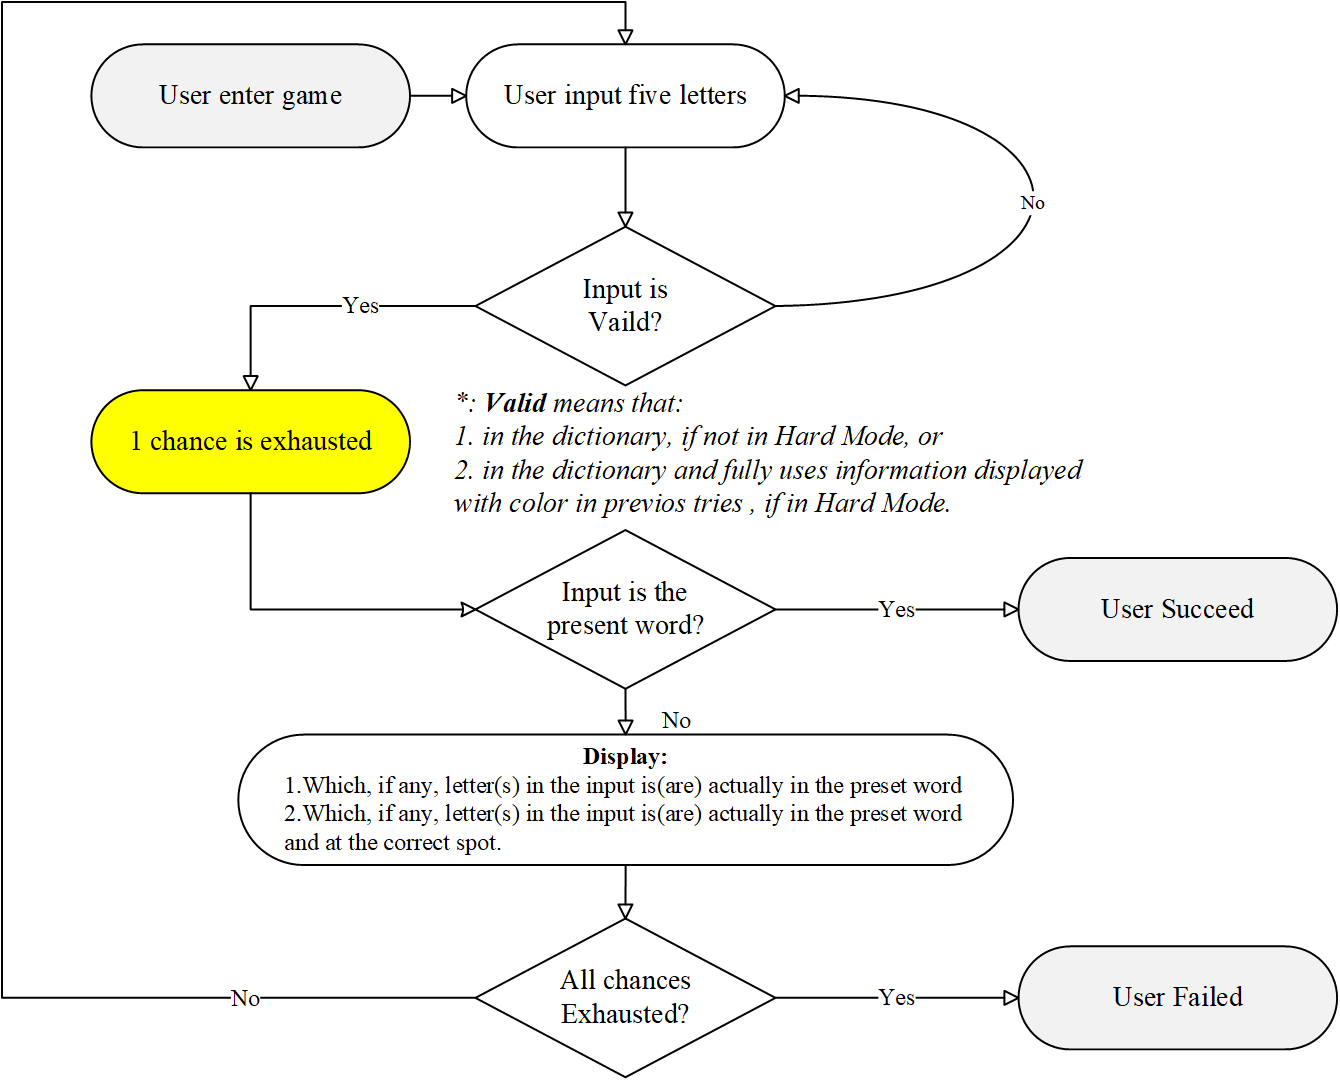
\includegraphics[width=14cm]{figure/2.png}  % 引入图片源
\caption{Rules} \label{Figure1}  % 标题与标签
\end{figure}  % 图片结束

\subsection{Restatement of the Problem}

We need to analyze the data provided by The New York Times and address the following tasks:
\begin{itemize}  % 无序列表
        \item \textbf{Problem 1:}Develop a model to explain the variations in the daily reported results and predict the 
        range of reported results for March 1, 2023. Additionally, analyze which word attributes influence 
        players' decisions to select Hard Mode.
        \item \textbf{Problem 2:}Build a prediction model to estimate the percentage distribution of results (1, 2, 3, 4, 5, 6, X) 
        for a future day, with specific predictions for "EERIE" on March 1, 2023, and assess the model's accuracy.
        \item \textbf{Problem 3:}Develop a classification model to categorize words by difficulty level and identify their attributes. 
        Conduct a detailed analysis for "EERIE" and evaluate the model's accuracy.
        \item \textbf{Problem 4:}Explore and describe any other interesting insights or patterns found within the data.
\end{itemize}  % 无序列表结束

\subsection{Our Work}

\section{Assumptions and Notations}  % 二级标题

\section{Model 1}  % 一级标题

\section{Model 2}  % 一级标题

\section{Model 3}  % 一级标题

\section{Interesting Findings}  % 一级标题

\section{Sensitivety Analysis}  % 一级标题

\section{Model Assessment}

\subsection{Strengths}
\subsection{Weaknesses}

\section{Letter}
%\begin{figure}[h]  % 图片
%\small
%\centering  % 居中
%\includegraphics[width=12cm]{example.eps}  % 引入图片源
%\caption{example} \label{fig:example}  % 标题与标签
%\end{figure}  % 图片结束

% This is Figure \eqref{fig:example}.  % 引用图表

% This is a cite\cite{vaswani2017attention}.  % 引用文献

\begin{equation}  % 公式,独占一行、居中,自动编号
E = mc^2 \label{aa}  % 标签
\end{equation}  % 公式结束

\begin{equation}  % 公式,独占一行、居中
\nonumber % 不编号
E = mc^2
\end{equation}  % 公式结束


\begin{itemize}  % 无序列表
        \item This is a item.
        \item This is a item.
\end{itemize}  % 无序列表结束


\begin{itemize}  % 无序列表
                \item This is a assumption.
                \item This is a assumption.
                \item This is a assumption.
                \item This is a assumption.
 \end{itemize}  % 无序列表结束

 \textit{I love math.}  % 斜体

\textbf{I love math.}  % 粗体

\underline{I love math.}  %下划线
%%%%%%%%%%%%%%%%%%%%%%%% 并排图 %%%%%%%%%%%%%%%%%%%%%%%%
%\begin{figure}[h]  % 图片
%\centering  % 居中
%\begin{minipage}[c]{0.48\textwidth}  % 子页
%\centering  % 居中
%\includegraphics[width=7cm]{example.eps}  % 引入图片源
%\caption{example} \label{fig:example}  % 标题与标签
%\end{minipage}  % 子页结束
%\hspace{0.02\textwidth}
%\begin{minipage}[c]{0.48\textwidth}  % 子页
%\centering  % 居中
%\includegraphics[width=7cm]{example.eps}  % 引入图片源
%\caption{example} \label{fig:example}  % 标题与标签
%\end{minipage}  % 子页结束
%\end{figure}  % 图片结束
%%%%%%%%%%%%%%%%%%%%%% 并排图结束 %%%%%%%%%%%%%%%%%%%%%%

%%%%%%%%%%%%%%%%%%%%%%%% 三线表 %%%%%%%%%%%%%%%%%%%%%%%%
\begin{table}[!t]  % 表格
\caption{Caption}  % 标题
\label{tab1}  % 标签
\tabcolsep 42pt % 列间距
\begin{tabular*}{\textwidth}{cccc}  % tabular*环境
\toprule  % 顶线
Title a & Title b & Title c & Title d \\
\midrule  % 中线
Aaa & Bbb & Ccc & Ddd \\
Aaa & Bbb & Ccc & Ddd \\
Aaa & Bbb & Ccc & Ddd \\
\bottomrule  % 底线
\end{tabular*}  % tabular*环境结束
\end{table}  % 表格结束
%%%%%%%%%%%%%%%%%%%%%% 三线表结束 %%%%%%%%%%%%%%%%%%%%%%


\printbibliography  % 打印引用文献列表

%%%%%%%%%%%%%%%%%%%%%%% 正文结束 %%%%%%%%%%%%%%%%%%%%%%%

\begin{appendices}  % 附录

\begin{memo}[Memorandum]  % 建议书
	This is a memorandum.
\end{memo}  % 建议书结束

\section{First appendix}  % 一级标题

Here are simulation programmes we used in our model as follow.\\
\textbf{MATLAB source code:}
%\lstinputlisting[language=Matlab]{./code/matlab.m}

\section{Second appendix}  % 一级标题

\textbf{Python source code:}
%\lstinputlisting[language=C++]{./code/python.py}

\end{appendices}  % 附录结束
\end{document}  % 文档结束
%%%%%%%%%%%%%%%%%%%%%%%%%%%%%%%%%%%%%%%%%%%%%%%%%%%%%%%